Una vez instalado y puesto en funcionamiento Netdata, el monitoreo puede realizarse de
dos maneras. La primera consiste en acceder directamente al agente mediante la dirección
IP de la Raspberry Pi y el puerto TCP 19999:

\begin{center}
\texttt{http://DIRECCION-IP:19999}
\end{center}

Este panel local permite consultar las métricas recopiladas por el agente, como el uso del
procesador, memoria, almacenamiento, interfaces de red, procesos y servicios. Sin
embargo, el panel local no está diseñado para crear cuentas individuales ni administrar
permisos para diferentes equipos de trabajo.

Para disponer de usuarios, roles, grupos de infraestructura y tableros compartidos, el
agente debe conectarse a Netdata Cloud. Esta plataforma proporciona una interfaz
centralizada desde la cual es posible organizar los dispositivos supervisados y controlar
qué información puede consultar o modificar cada integrante del equipo.

\section{Conexión del agente con Netdata Cloud}

Primero se debe crear una cuenta en Netdata Cloud ingresando a:

\begin{center}
\url{https://app.netdata.cloud}
\end{center}

La cuenta utilizada para crear el entorno será la cuenta principal o administradora. Una
vez iniciada la sesión, se debe crear un \textit{Space}. Un Space representa el entorno
principal de colaboración y contiene los usuarios, nodos, salas y dashboards de la
organización.

Para conectar el agente instalado en la Raspberry Pi se pueden seguir estos pasos:

\begin{enumerate}
    \item Abrir el panel local mediante \texttt{http://DIRECCION-IP:19999}.
    \item Iniciar sesión con la cuenta de Netdata Cloud.
    \item Seleccionar la opción \textit{Connect}.
    \item Seguir las instrucciones mostradas para comprobar que se posee acceso
          administrativo a la Raspberry Pi.
    \item Seleccionar el Space al cual se conectará el nodo.
\end{enumerate}

Después de completar el procedimiento, la Raspberry Pi aparecerá como un nodo dentro
del Space. La conexión entre el agente y Netdata Cloud se realiza mediante el
\textit{Agent-Cloud Link} y utiliza una conexión saliente cifrada por el puerto TCP 443.

\begin{figure}[H]
    \centering
    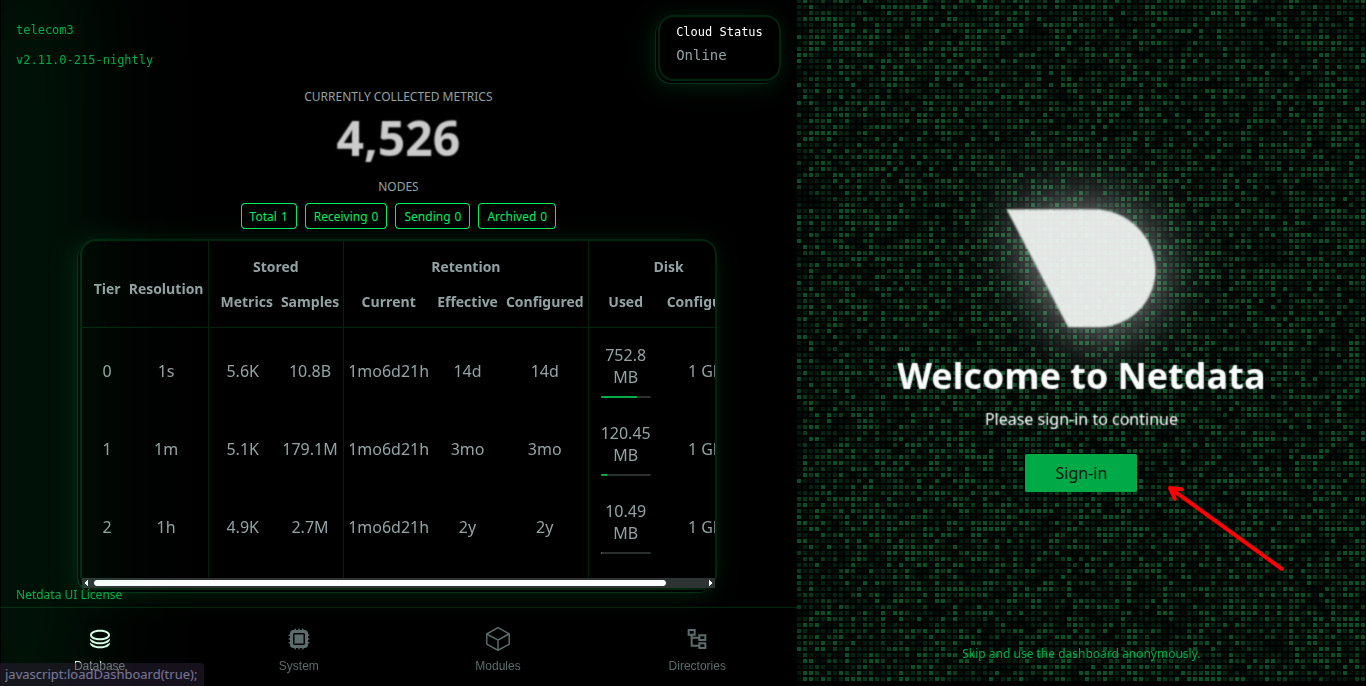
\includegraphics[scale= 0.35]{Pictures/7/1/0.png}
    \caption{Iniciar sesión: Google \textit{Account} por ejemplo}
    \label{CON1}
\end{figure}

\begin{figure}[H]
    \centering
    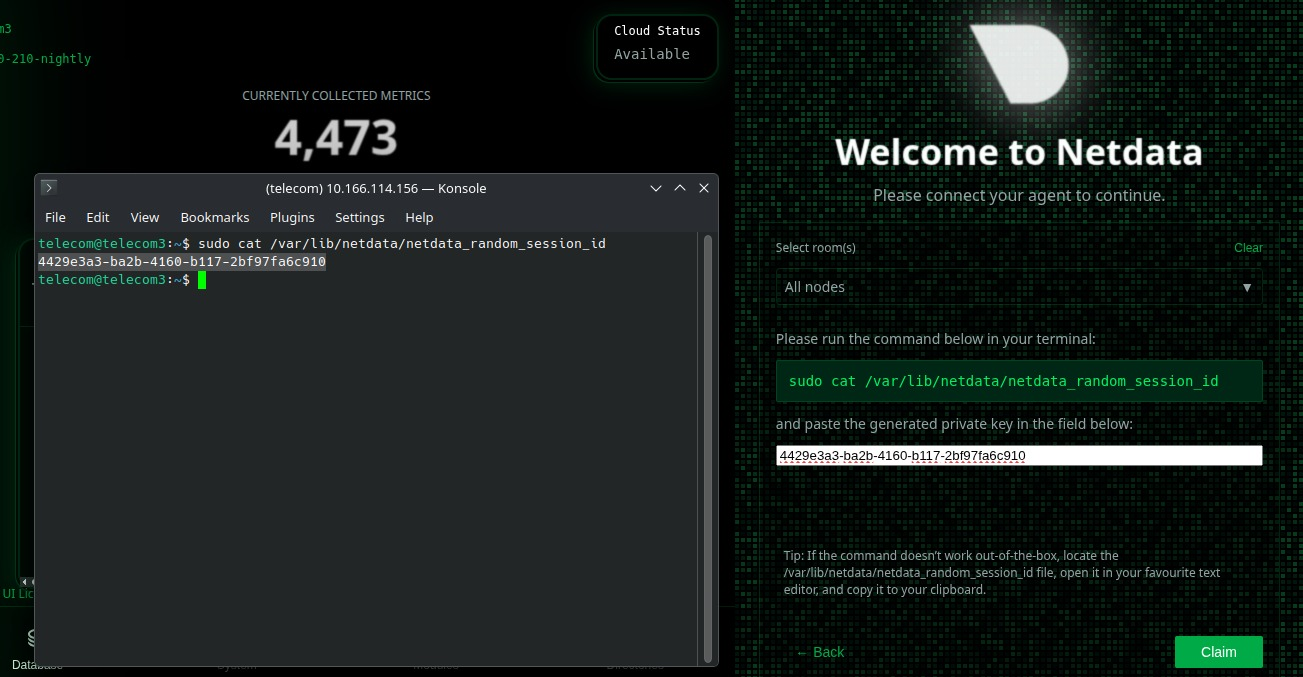
\includegraphics[scale= 0.25]{Pictures/7/1/1.jpeg}
    \caption{Se obtiene llave desde el sever}
    \label{CON1}
\end{figure}


\begin{figure}[H]
    \centering
    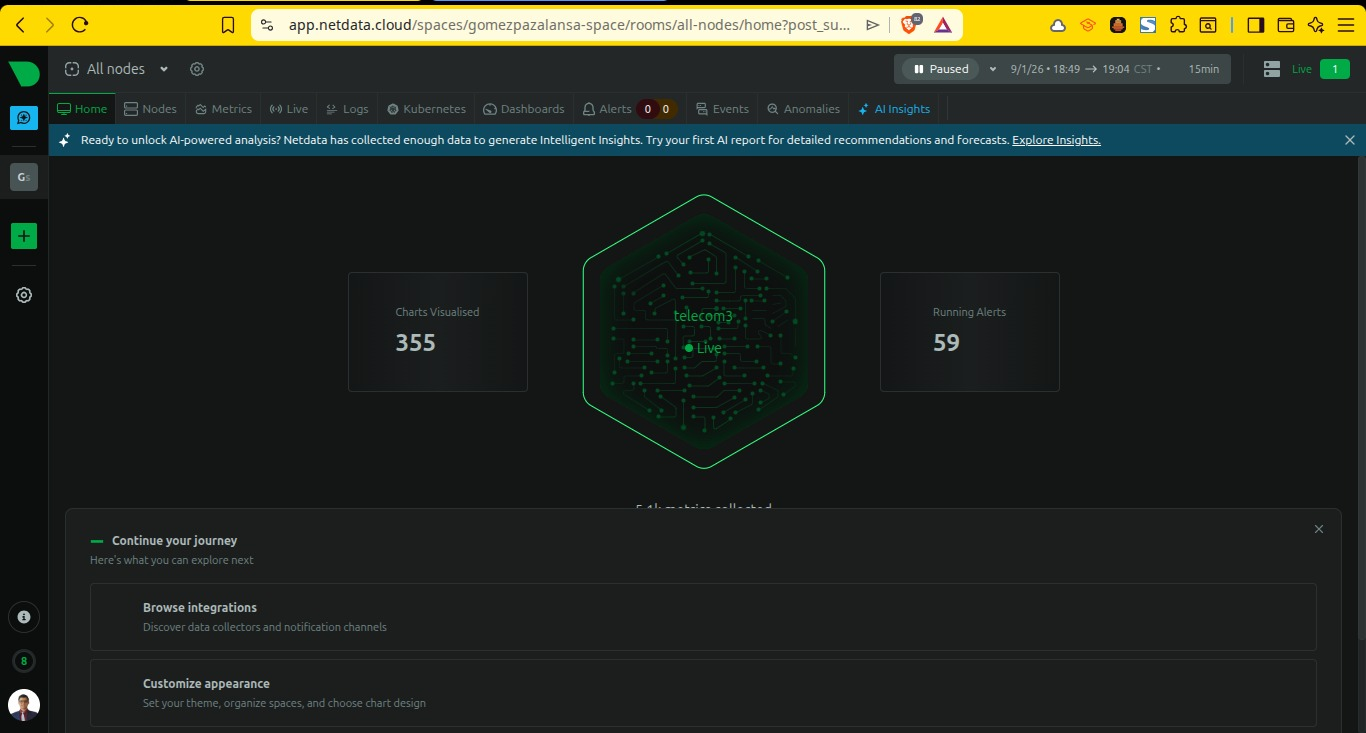
\includegraphics[scale= 0.25]{Pictures/7/1/2.jpeg}
    \caption{Netdata Only}
    \label{CON1}
\end{figure}

\begin{figure}[H]
    \centering
    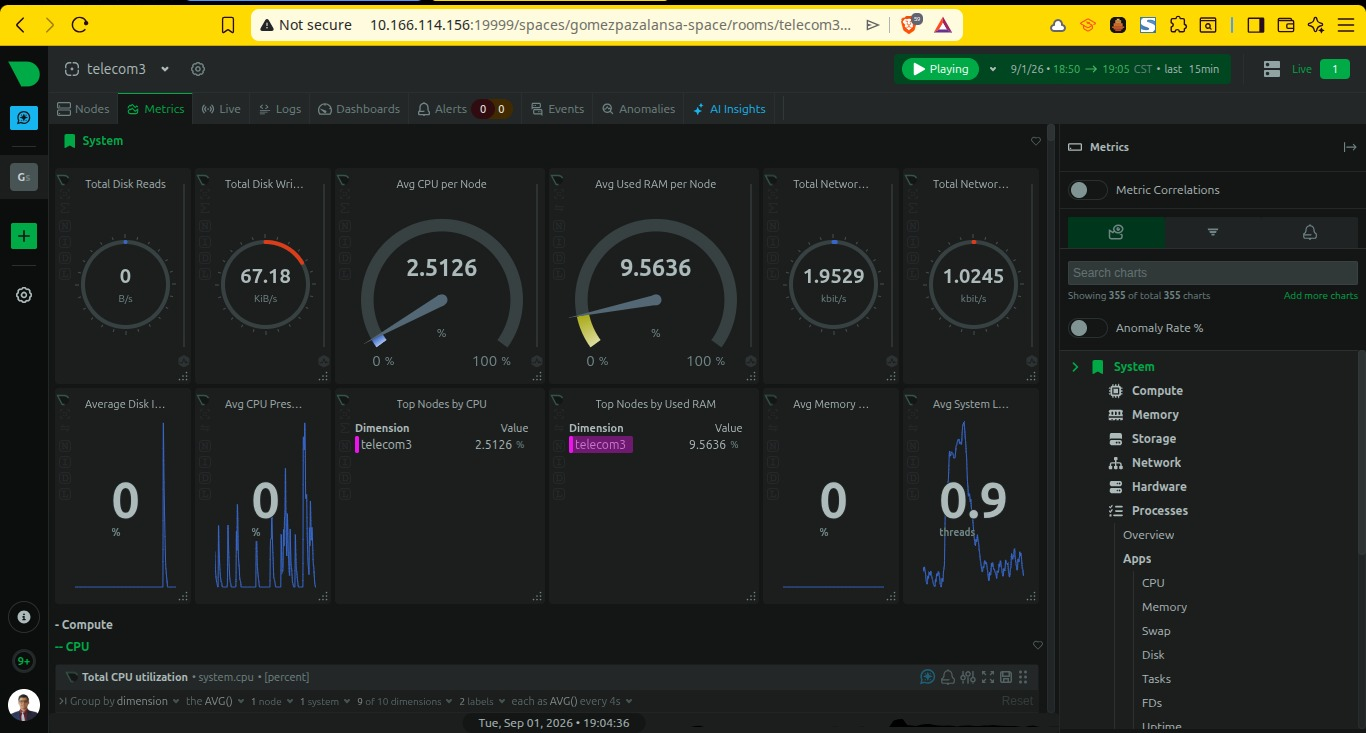
\includegraphics[scale= 0.25]{Pictures/7/1/3.jpeg}
    \caption{Pagina de configuración de Netdata}
    \label{CON1}
\end{figure}


\section{Gestión de usuarios}

La gestión de usuarios se realiza desde Netdata Cloud y no desde el panel local del
puerto 19999. La cuenta principal debe conservar el rol de \textit{Admin}, debido a que
este rol permite administrar el Space, los usuarios, los nodos, las salas y las
configuraciones generales.

Para consultar o modificar los usuarios se debe realizar lo siguiente:

\begin{enumerate}
    \item Seleccionar el Space correspondiente.
    \item Abrir \textit{Space Settings}, representado por el icono de engranaje.
    \item Seleccionar la pestaña \textit{User Management}.
    \item Localizar al usuario que se desea modificar.
    \item Asignar el rol correspondiente o eliminar su acceso cuando ya no sea necesario.
\end{enumerate}

Netdata Cloud utiliza un modelo de control de acceso basado en roles. Los principales
roles disponibles son:

\begin{description}
    \item[Admin:] posee control completo sobre el Space, los usuarios, los nodos, las
    salas, las configuraciones y la facturación. Se recomienda mantener este rol
    únicamente en la cuenta principal y en una cuenta administrativa de respaldo.

    \item[Manager:] puede administrar usuarios, salas y configuraciones operativas, pero
    no posee control sobre la facturación ni sobre determinadas opciones exclusivas del
    administrador.

    \item[Troubleshooter:] puede consultar métricas, investigar problemas, ejecutar
    diagnósticos permitidos y crear dashboards dentro de las salas asignadas.

    \item[Observer:] está orientado a usuarios que solamente necesitan consultar las
    métricas y dashboards de determinadas salas.

    \item[Billing:] permite administrar información de facturación, sin proporcionar
    acceso operativo a los sistemas monitoreados.
\end{description}

Los roles disponibles pueden variar según el plan contratado en Netdata Cloud. Por esta
razón, antes de diseñar la estructura de permisos debe comprobarse qué funciones están
incluidas en el plan utilizado.

\begin{figure}[H]
    \centering
    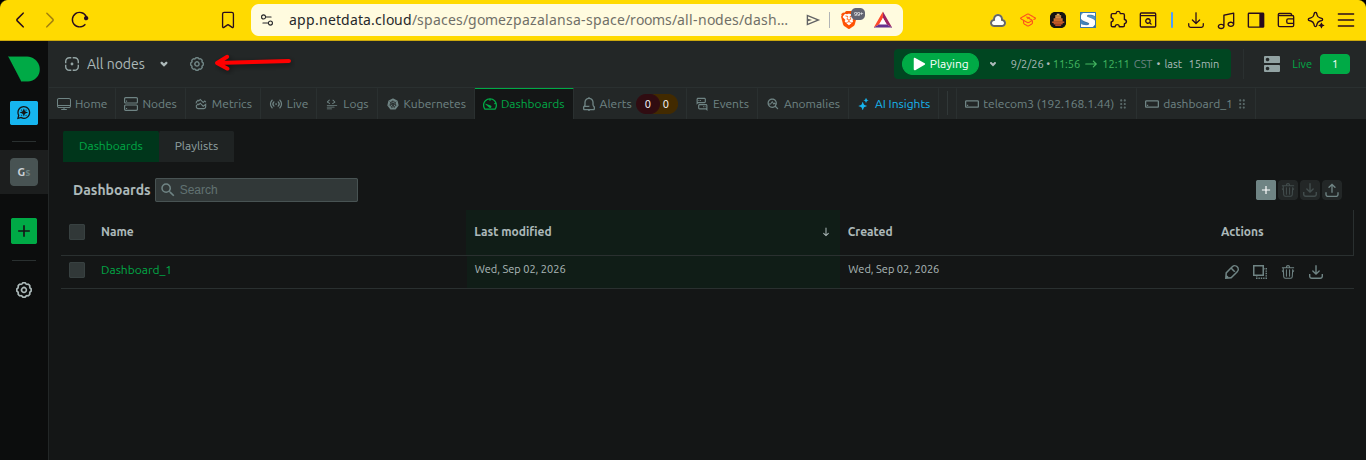
\includegraphics[scale= 0.4]{Pictures/7/2/0.png}
    \caption{Configuración de \textit{Space}}
    \label{CON1}
\end{figure}

\begin{figure}[H]
    \centering
    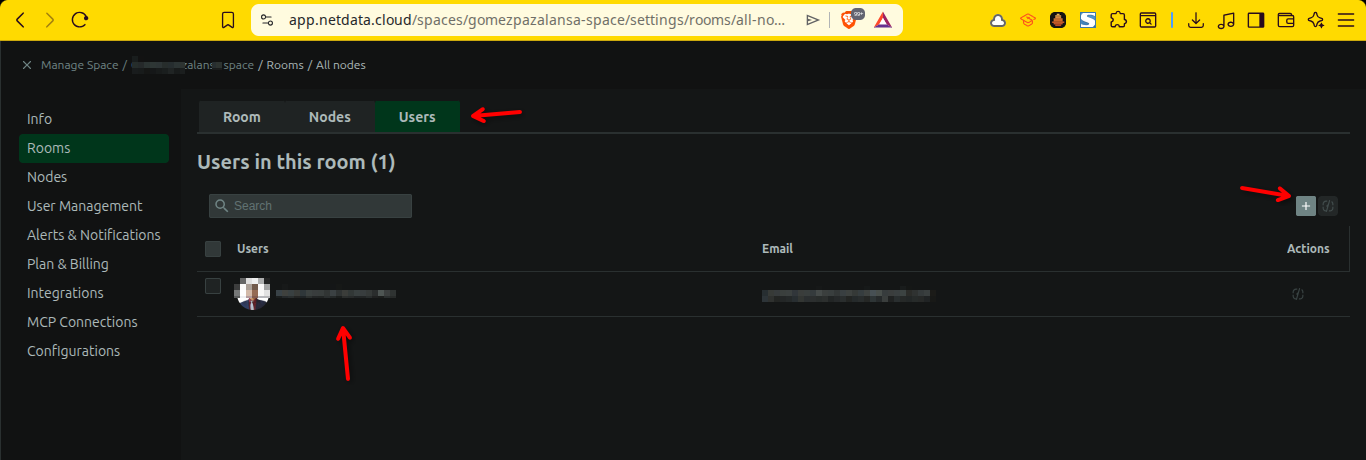
\includegraphics[scale= 0.4]{Pictures/7/2/1.png}
    \caption{Usuarios}
    \label{CON1}
\end{figure}

\begin{figure}[H]
    \centering
    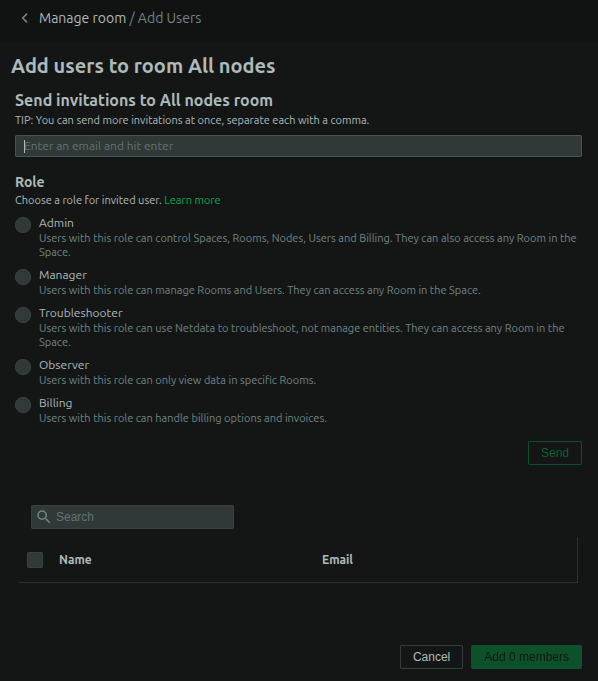
\includegraphics[scale= 0.4]{Pictures/7/2/2.png}
    \caption{\textit{Add User}}
    \label{CON1}
\end{figure}


\section{Creación de usuarios para los equipos de trabajo}

En Netdata Cloud no es recomendable crear una única cuenta y compartir su contraseña
entre todos los integrantes. Cada persona debe utilizar una cuenta individual asociada
con su dirección de correo electrónico.

Para agregar un usuario se debe realizar el siguiente procedimiento:

\begin{enumerate}
    \item Ingresar al Space con la cuenta principal.
    \item Seleccionar la opción \textit{Invite Users}.
    \item Escribir la dirección de correo electrónico del integrante.
    \item Seleccionar el rol que tendrá dentro del Space.
    \item Enviar la invitación.
    \item Esperar a que el usuario acepte la invitación y complete la creación de su
          cuenta.
\end{enumerate}

Para separar al personal de IT, Cloud e Infraestructura se pueden crear diferentes
\textit{Rooms}. Una Room es una agrupación lógica de nodos, dashboards y usuarios
dentro de un Space. Por ejemplo, se puede utilizar la siguiente estructura:

\begin{itemize}
    \item \textbf{IT:} servidores y servicios administrados por el equipo de tecnología.
    \item \textbf{Cloud:} máquinas virtuales, contenedores y servicios desplegados en la
          nube.
    \item \textbf{Infraestructura:} equipos físicos, almacenamiento, enlaces y
          dispositivos de red.
\end{itemize}

Para crear una Room se debe seleccionar el símbolo más ubicado junto a la opción
\textit{Rooms}, asignarle un nombre y agregar los nodos correspondientes. Posteriormente,
desde la configuración de la Room, un administrador o manager puede agregar los
usuarios que necesitan acceso.

Un mismo nodo puede pertenecer a varias Rooms, pero solamente puede estar asociado con
un Space. Esto permite que la Raspberry Pi o cualquier otro servidor sea visible para
más de un equipo sin tener que instalar nuevamente el agente.

\begin{figure}[H]
    \centering
    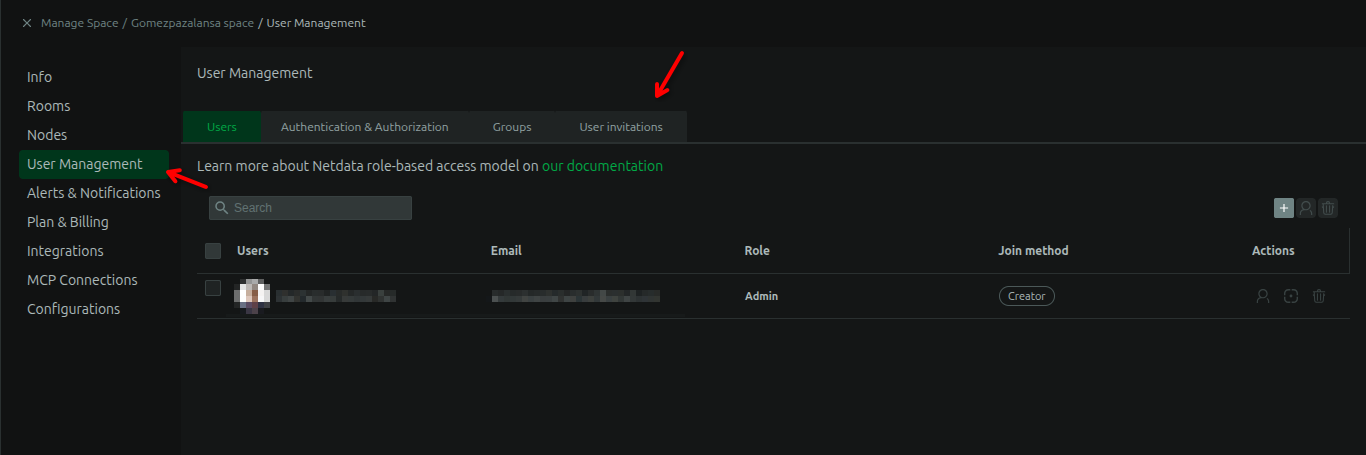
\includegraphics[scale= 0.4]{Pictures/7/3/1.png}
    \caption{\textit{User Managment}}
    \label{CON1}
\end{figure}

\begin{figure}[H]
    \centering
    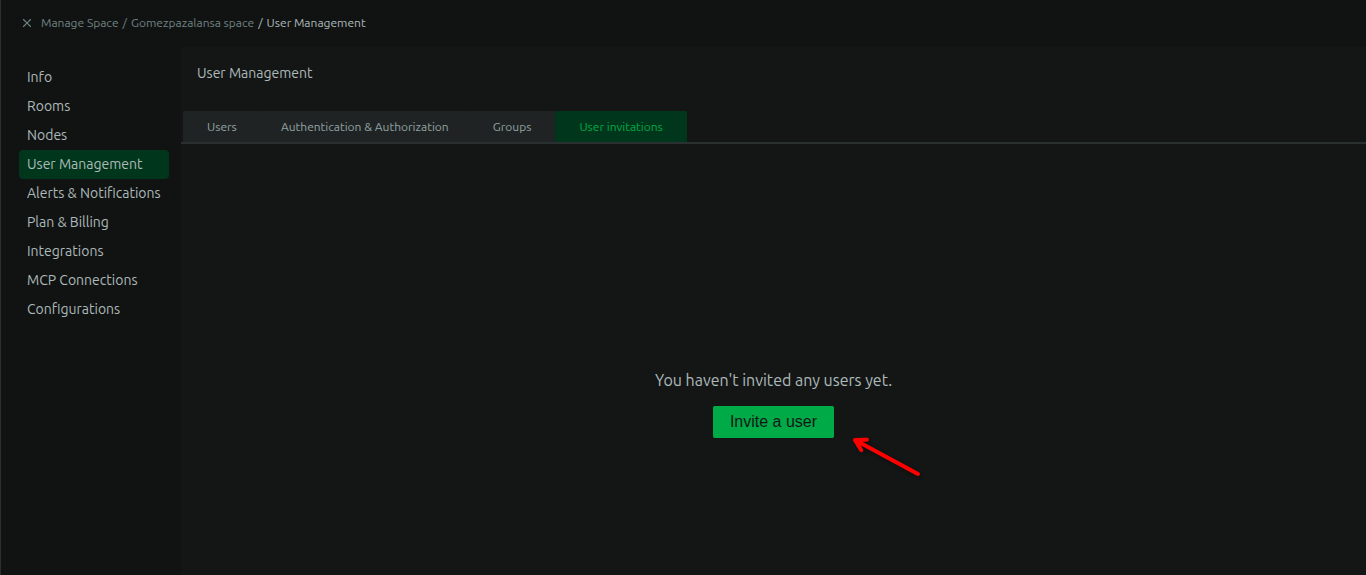
\includegraphics[scale= 0.4]{Pictures/7/3/2.png}
    \caption{\textit{User invitations}}
    \label{CON1}
\end{figure}

\begin{figure}[H]
    \centering
    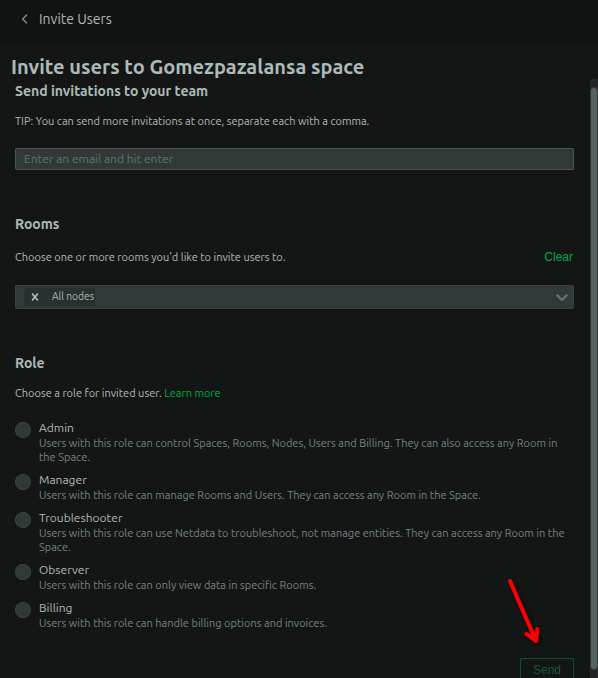
\includegraphics[scale= 0.4]{Pictures/7/3/3.png}
    \caption{\textit{Send invite}}
    \label{CON1}
\end{figure}


\section{Credenciales y contraseñas}

La cuenta principal no crea manualmente las contraseñas de los demás integrantes. El
administrador únicamente envía una invitación a la dirección de correo electrónico de
cada usuario. Al aceptar la invitación, el usuario crea y administra sus propias
credenciales.

Netdata Cloud permite iniciar sesión mediante:

\begin{itemize}
    \item correo electrónico y contraseña;
    \item una cuenta de Google;
    \item una cuenta de GitHub;
    \item inicio de sesión empresarial o SSO, cuando el plan utilizado lo permite.
\end{itemize}

Por seguridad, no se deben compartir contraseñas ni utilizar una cuenta genérica para
todo un departamento. Cada integrante debe poseer una cuenta individual, ya que esto
permite retirar únicamente su acceso cuando abandona el equipo y facilita identificar
las acciones realizadas dentro de la plataforma.

La contraseña debe crearse únicamente en la página oficial de Netdata Cloud. No debe
almacenarse en documentos, scripts, archivos de configuración ni mensajes enviados al
equipo. También se recomienda utilizar contraseñas diferentes para cada cuenta y
habilitar los mecanismos de seguridad disponibles en el proveedor de autenticación.

Las credenciales personales no deben confundirse con el \textit{claiming token} utilizado
para conectar un agente con un Space. Este token es una credencial administrativa y
debe tratarse como información confidencial. No se debe incluir en el manual, en
capturas de pantalla ni en repositorios de código.

% \begin{figure}[H]
%     \centering
%     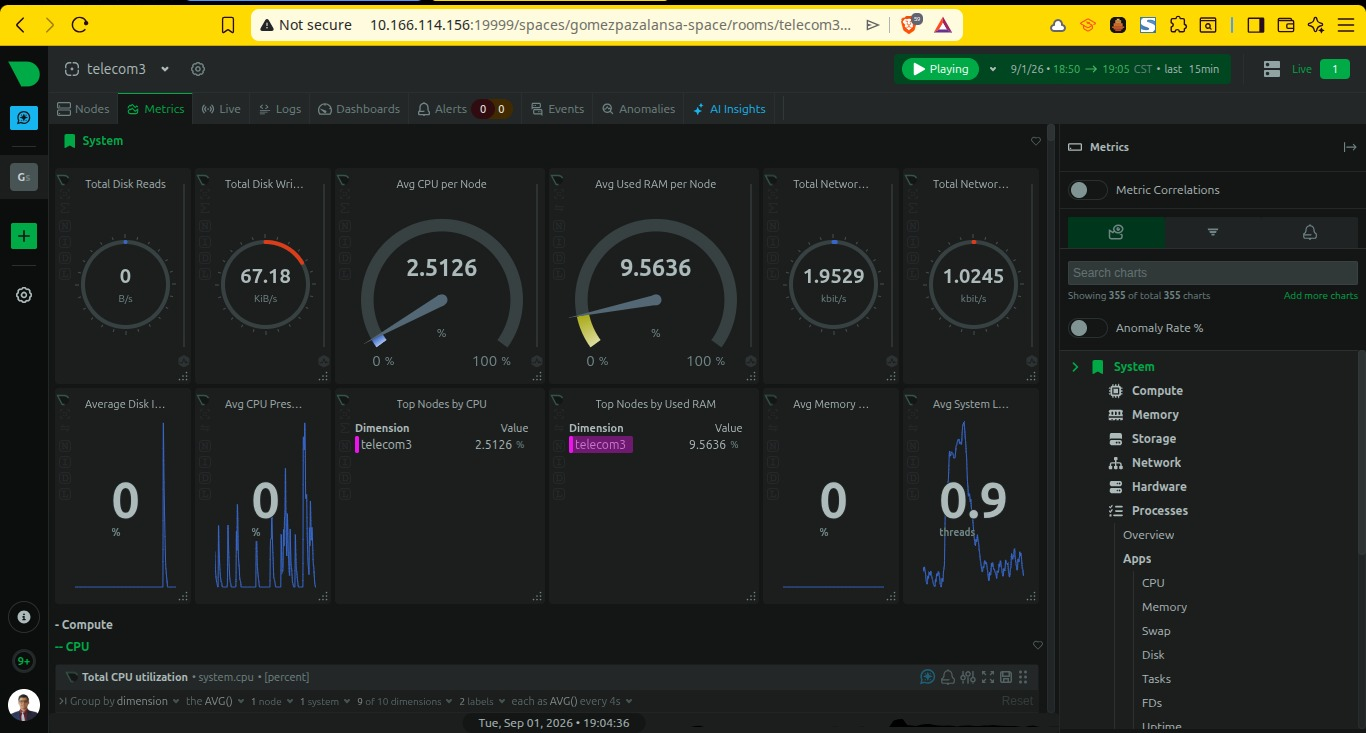
\includegraphics[scale= 0.25]{Pictures/7/1/3.jpeg}
%     \caption{Pagina de configuración de Netdata}
%     \label{CON1}
% \end{figure}


\section{Creación de dashboards}

Los dashboards permiten reunir en una sola pantalla las métricas más importantes para
un equipo o servicio. Cada dashboard pertenece a una Room, por lo que solamente los
usuarios con acceso a esa Room podrán utilizarlo.

Para crear un dashboard se debe seguir este procedimiento:

\begin{enumerate}
    \item Seleccionar la Room en la que se desea crear el dashboard.
    \item Abrir la pestaña \textit{Dashboards}.
    \item Presionar el botón con el símbolo más.
    \item Escribir un nombre descriptivo y seleccionar \textit{Add}.
    \item Presionar \textit{Add Chart} para agregar una gráfica.
    \item Seleccionar todos los nodos o un nodo específico como fuente.
    \item Seleccionar el contexto o métrica que se desea representar.
    \item Configurar las dimensiones, filtros, agrupaciones y tipo de gráfica.
    \item Organizar y cambiar el tamaño de las gráficas mediante las opciones de
          arrastrar y soltar.
    \item Presionar \textit{Save} para guardar los cambios.
\end{enumerate}

También se pueden agregar tarjetas de texto mediante la opción \textit{Add Text}. Estas
tarjetas permiten documentar el propósito del dashboard, explicar valores esperados o
registrar instrucciones para responder ante una alerta.

Como ejemplo, el dashboard del equipo de Infraestructura puede incluir las siguientes
métricas:

\begin{itemize}
    \item porcentaje de utilización del procesador;
    \item memoria RAM utilizada y disponible;
    \item capacidad y actividad de los dispositivos de almacenamiento;
    \item tráfico recibido y transmitido por las interfaces de red;
    \item temperatura de la Raspberry Pi;
    \item cantidad de alertas activas;
    \item estado de los servicios supervisados.
\end{itemize}

Los dashboards de Netdata son paneles interactivos y no equivalen necesariamente a un
reporte estático en formato PDF. Permiten modificar el intervalo de tiempo, ampliar una
sección de las gráficas y comparar datos de varios nodos. Si se necesita conservar una
evidencia estática, se puede utilizar la función de impresión o exportación del navegador
para generar un archivo PDF.

Netdata Cloud también dispone de un modo denominado \textit{TV Mode}, destinado a
mostrar dashboards en pantallas compartidas. La dirección generada por este modo
contiene un token de acceso, por lo que debe tratarse como una credencial confidencial y
compartirse únicamente con personal autorizado.

\begin{figure}[H]
    \centering
    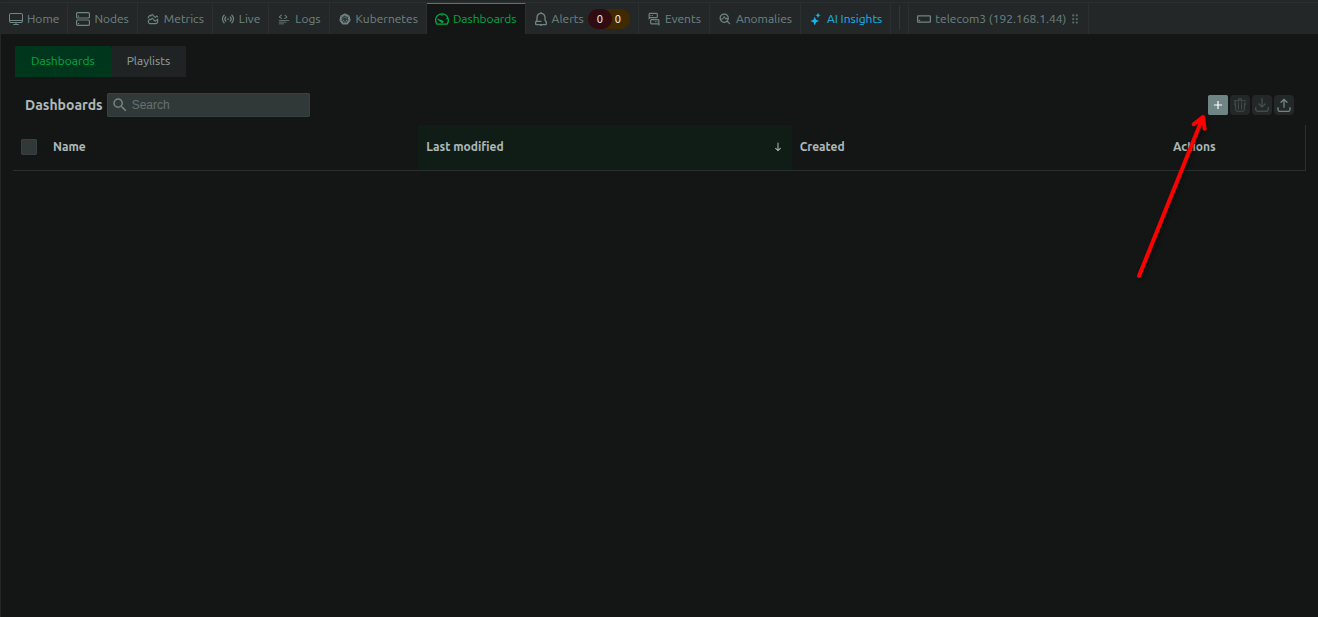
\includegraphics[scale= 0.4]{Pictures/7/5/1.png}
    \caption{Nuevo \textit{Dashboard}}
    \label{CON1}
\end{figure}

\begin{figure}[H]
    \centering
    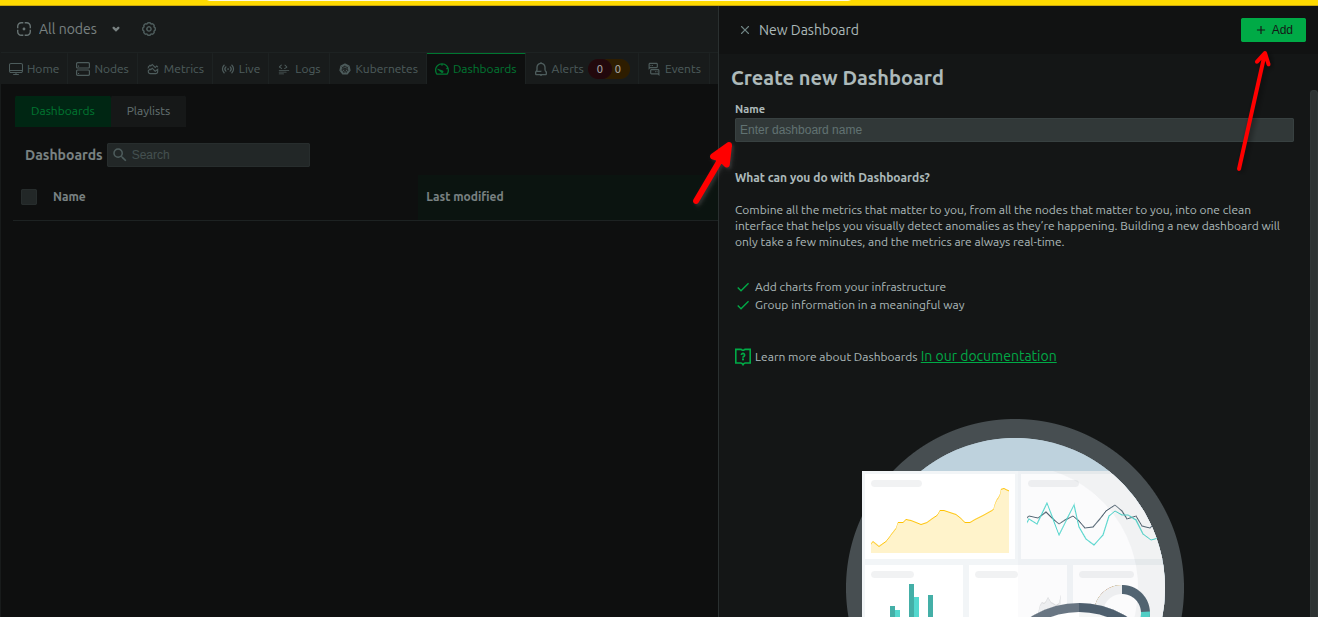
\includegraphics[scale= 0.4]{Pictures/7/5/2.png}
    \caption{Se le coloca nombre y \textit{Add}}
    \label{CON1}
\end{figure}


\begin{figure}[H]
    \centering
    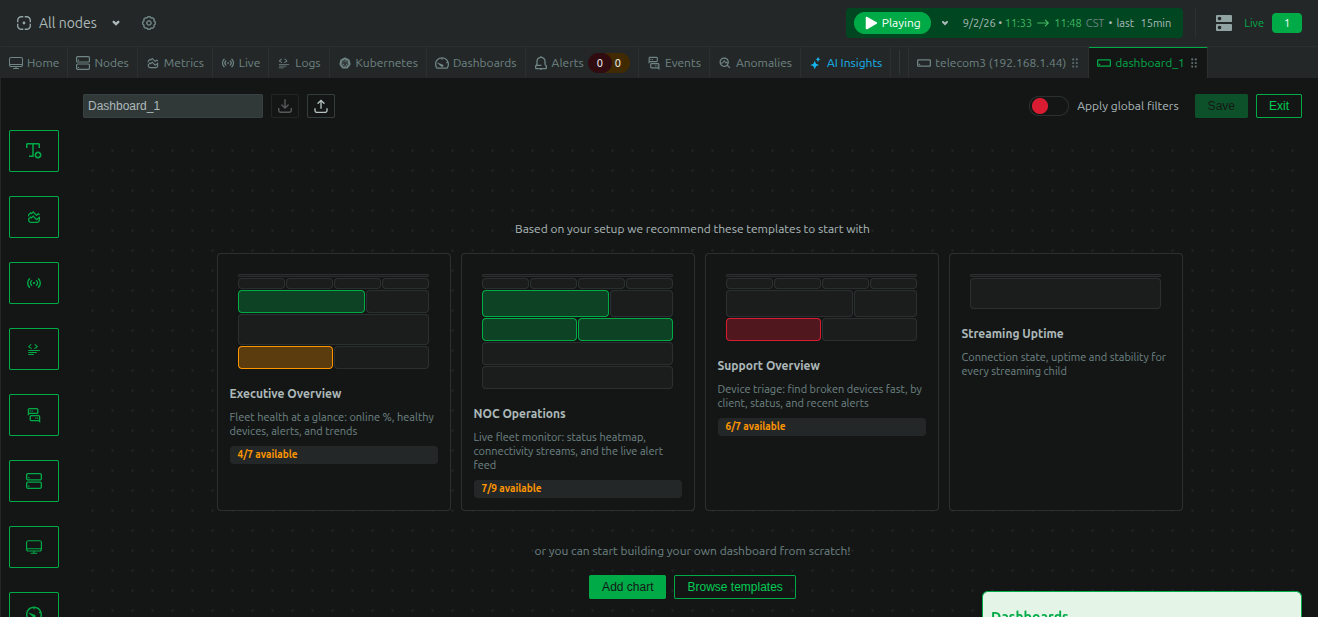
\includegraphics[scale= 0.4]{Pictures/7/5/3.png}
    \caption{Se pueden hacer nuevos \textit{templates} o diseñar uno desde 0}
    \label{CON1}
\end{figure}

\begin{figure}[H]
    \centering
    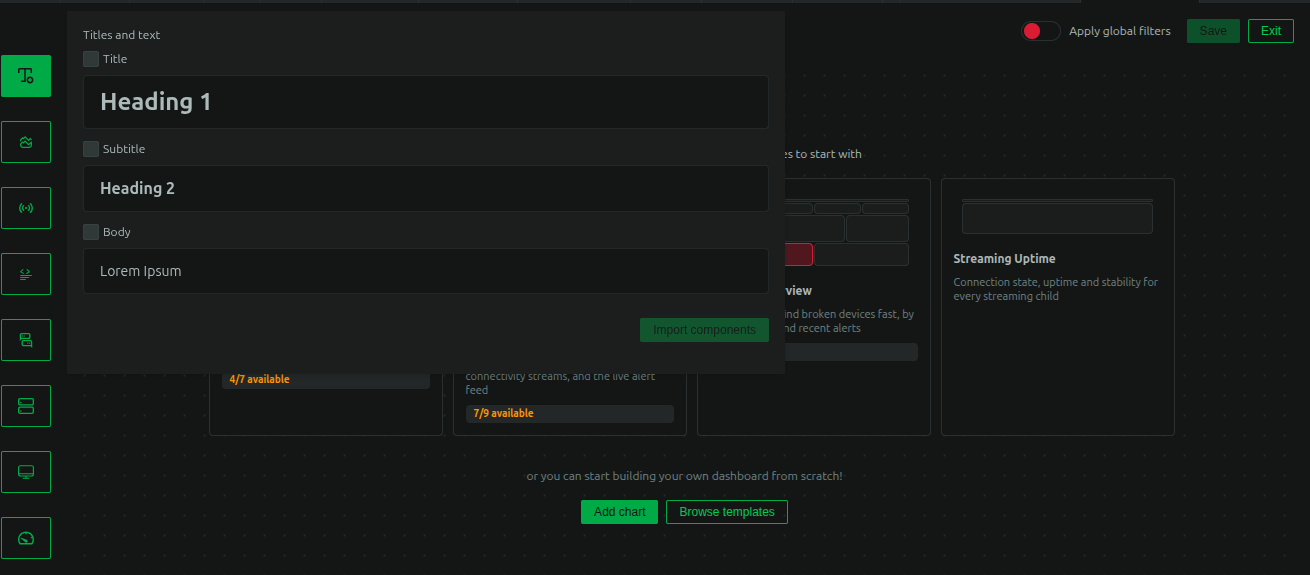
\includegraphics[scale= 0.4]{Pictures/7/5/4.png}
    \caption{\textit{Titles and text}}
    \label{CON1}
\end{figure}

\begin{figure}[H]
    \centering
    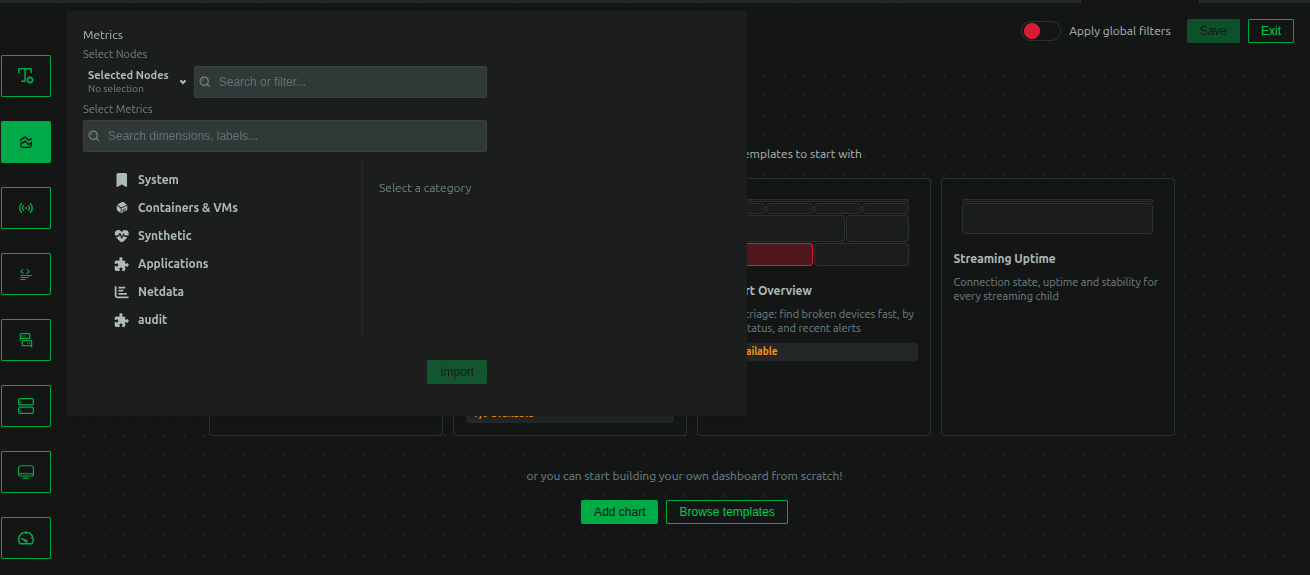
\includegraphics[scale= 0.4]{Pictures/7/5/5.png}
    \caption{\textit{Metrics}}
    \label{CON1}
\end{figure}


\begin{figure}[H]
    \centering
    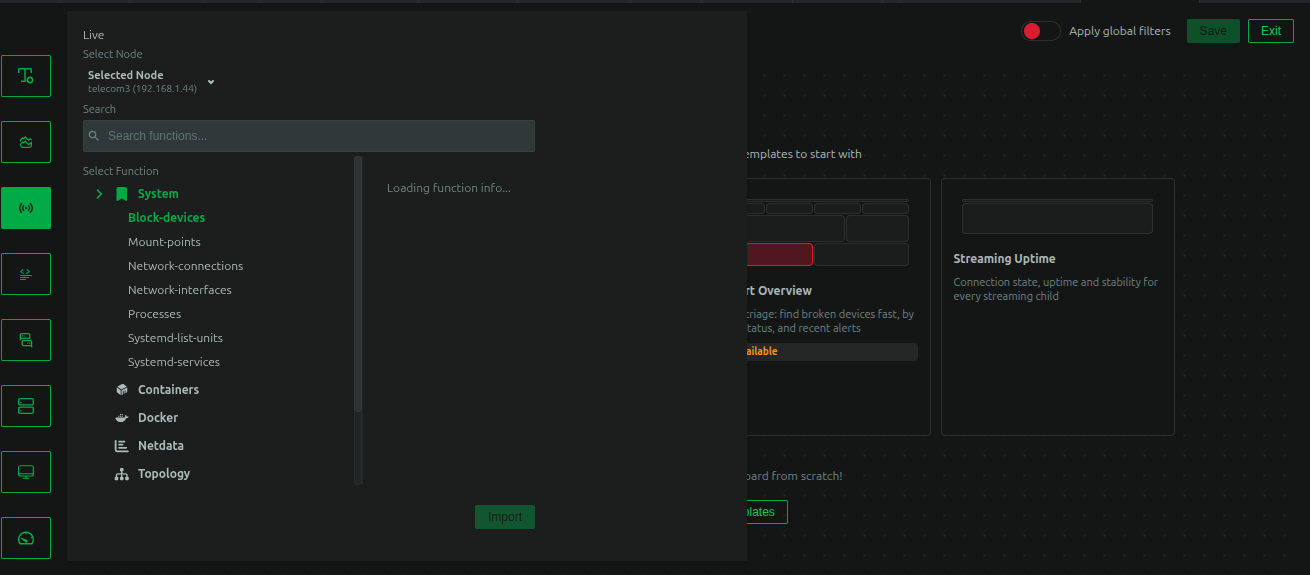
\includegraphics[scale= 0.4]{Pictures/7/5/6.png}
    \caption{\textit{Live}}
    \label{CON1}
\end{figure}

\begin{figure}[H]
    \centering
    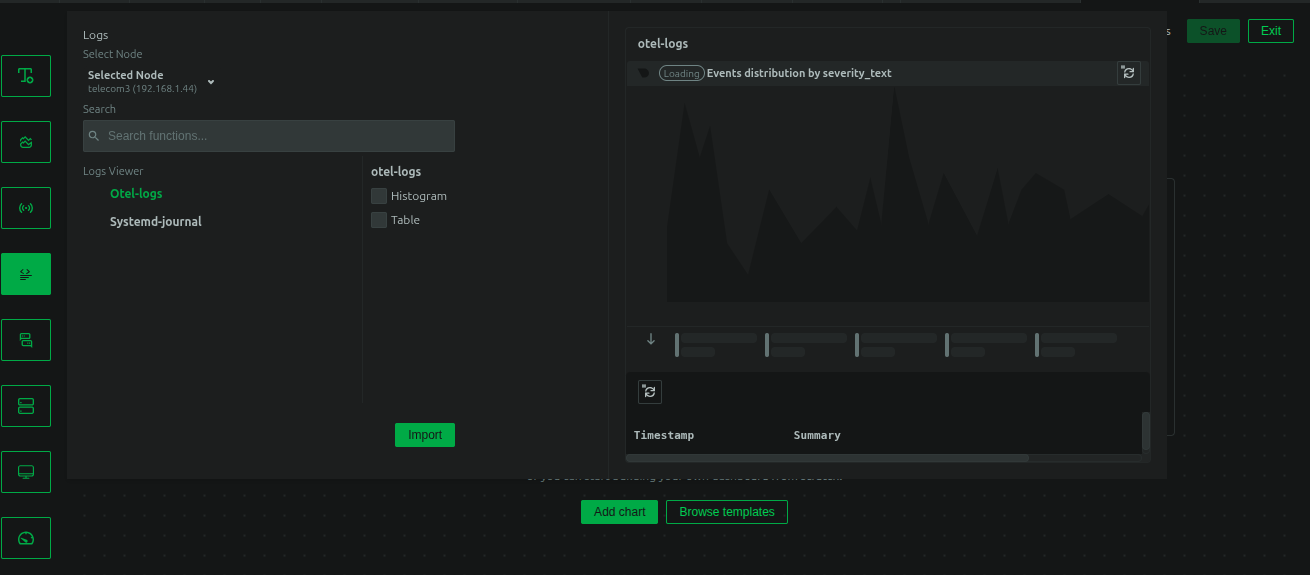
\includegraphics[scale= 0.4]{Pictures/7/5/7.png}
    \caption{\textit{Logs}}
    \label{CON1}
\end{figure}

\begin{figure}[H]
    \centering
    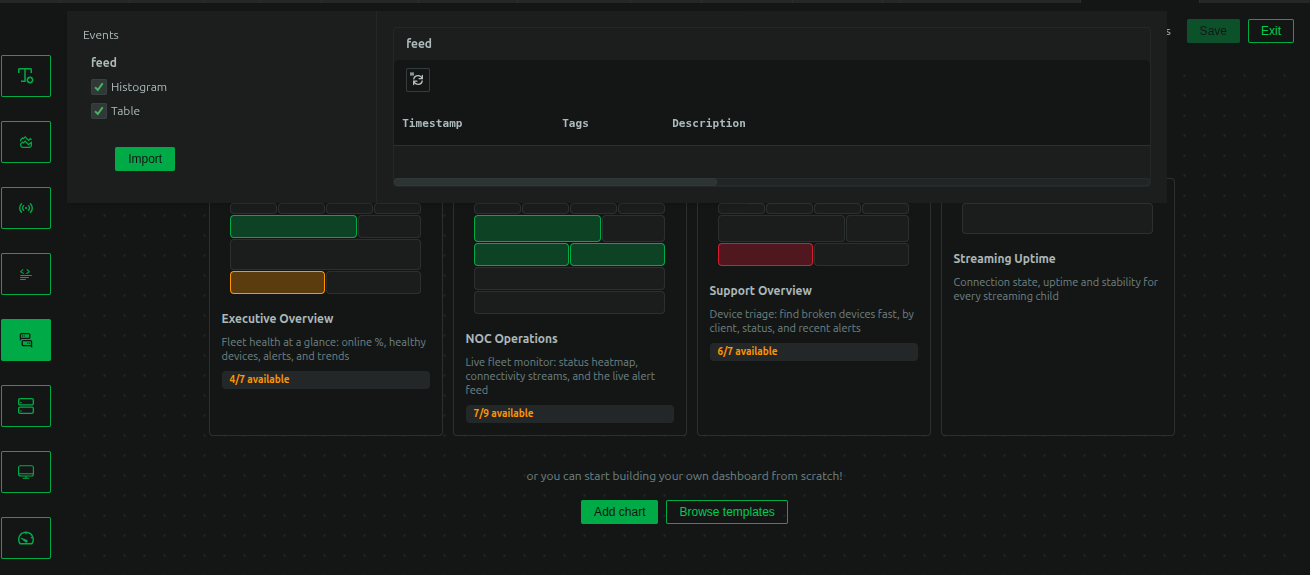
\includegraphics[scale= 0.4]{Pictures/7/5/8.png}
    \caption{\textit{Events}}
    \label{CON1}
\end{figure}


\begin{figure}[H]
    \centering
    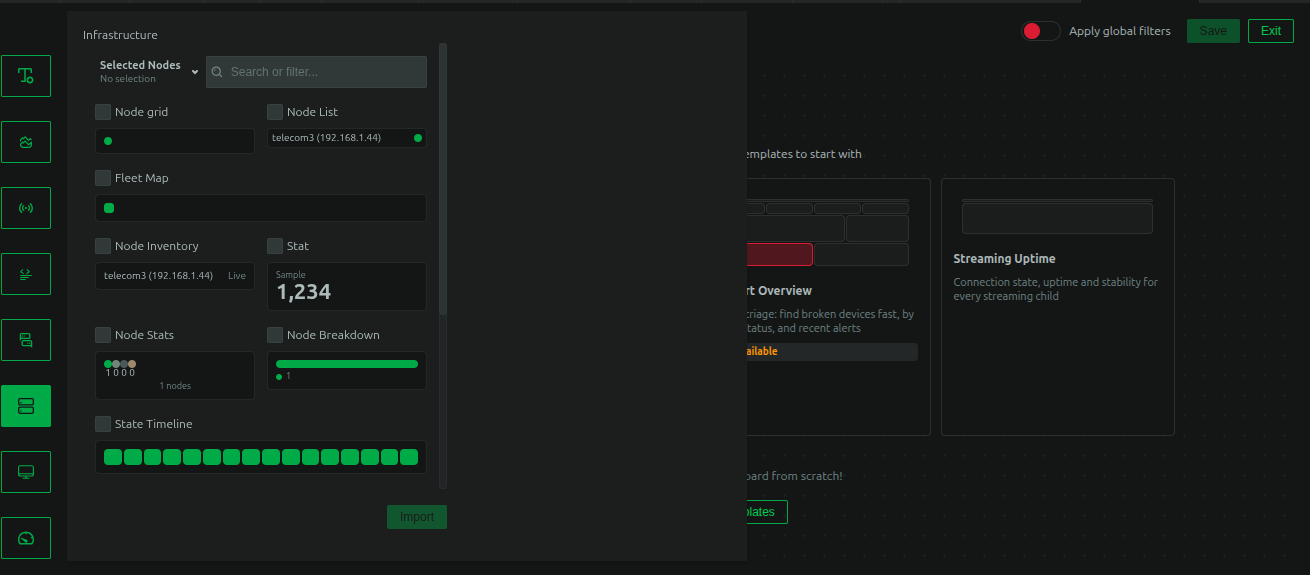
\includegraphics[scale= 0.4]{Pictures/7/5/9.png}
    \caption{\textit{Infrastructure}}
    \label{CON1}
\end{figure}

\begin{figure}[H]
    \centering
    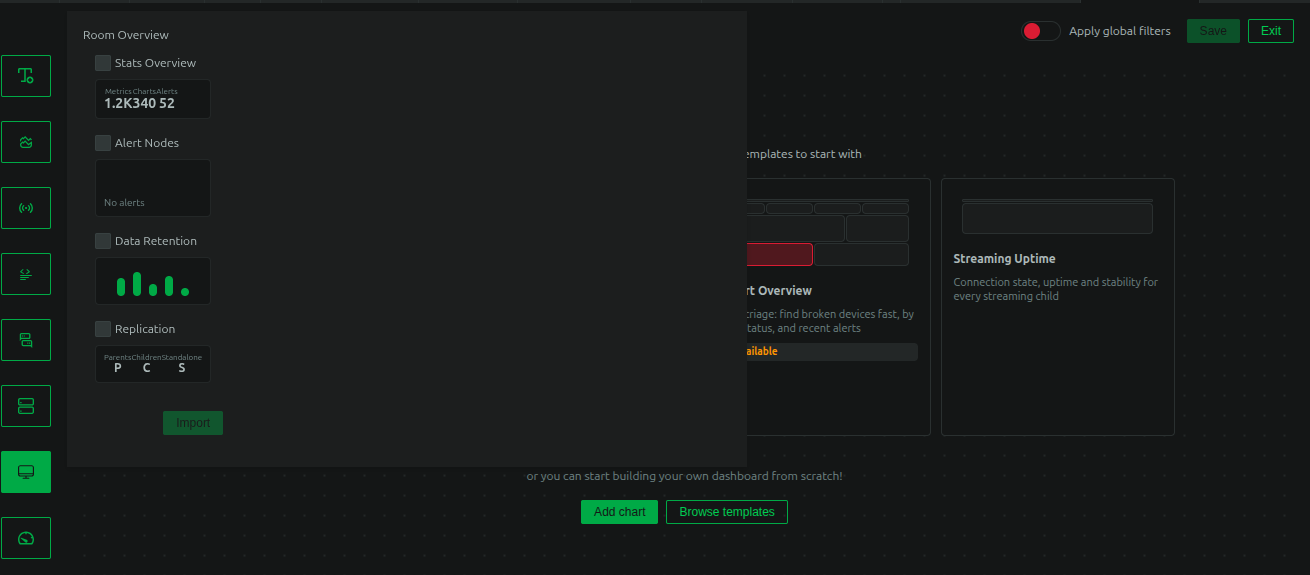
\includegraphics[scale= 0.4]{Pictures/7/5/10.png}
    \caption{\textit{Room Overview}}
    \label{CON1}
\end{figure}

\begin{figure}[H]
    \centering
    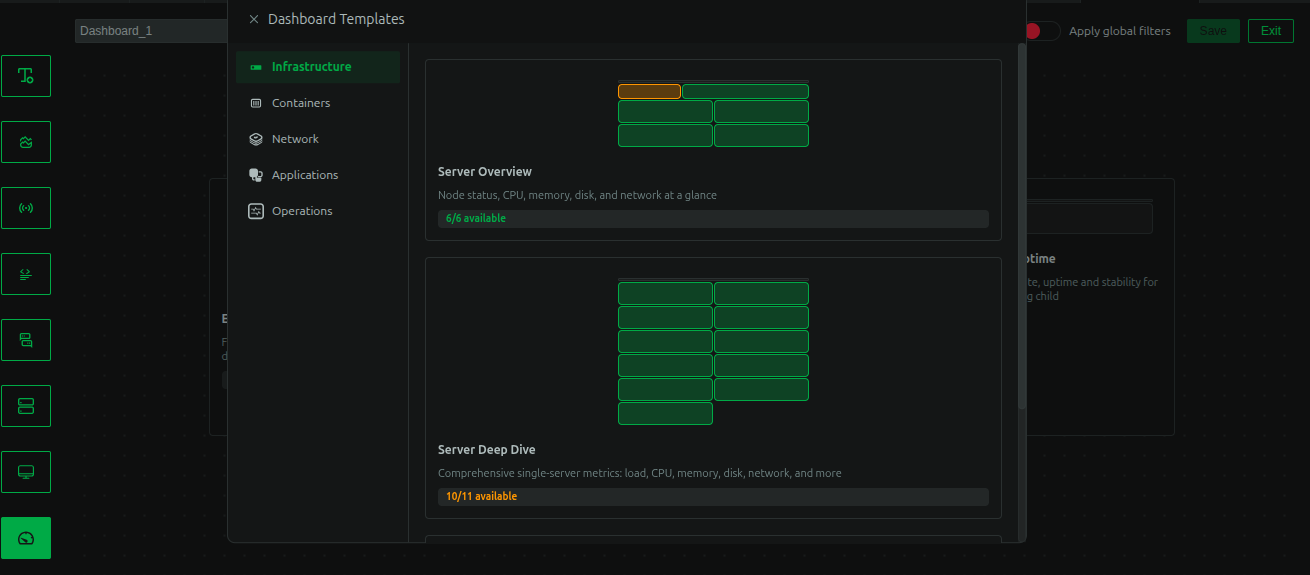
\includegraphics[scale= 0.4]{Pictures/7/5/11.png}
    \caption{\textit{Dashboard Templates}}
    \label{CON1}
\end{figure}


\section{Recomendaciones de administración}

Para mantener un entorno organizado y seguro se recomienda aplicar las siguientes
prácticas:

\begin{itemize}
    \item conservar una sola cuenta principal con privilegios administrativos y una
          cuenta de respaldo controlada;
    \item proporcionar a cada usuario solamente los permisos necesarios;
    \item utilizar Rooms separadas para IT, Cloud e Infraestructura;
    \item evitar el uso de cuentas y contraseñas compartidas;
    \item revisar periódicamente los usuarios y retirar accesos que ya no sean
          necesarios;
    \item no publicar tokens de conexión o enlaces de TV Mode;
    \item utilizar nombres descriptivos para los nodos, las Rooms y los dashboards;
    \item guardar los dashboards después de cada modificación.
\end{itemize}

De esta forma, la cuenta principal conserva el control administrativo, mientras que cada
equipo puede consultar o administrar únicamente los recursos necesarios para cumplir
sus funciones.